\chapter{Particle Accelerator Physics}\label{chap:2}
%
%
% The history of particle accelerators goes back to the 1930s when the first accelerators were designed to provide the particle energies required to study atomic nuclei. Nowadays, a vast variety of accelerator types is available for many different applications, reaching from low-energy machines for particle therapy in cancer treatment (for example Heidelberger Ionenstrahl-Therapiezentrum, HIT~\cite{HITref01}) over synchrotron light sources at intermediate energies (for example SOLEIL~\cite{SOLEILref01}) to high-energy synchrotron colliders for fundamental research, such as the Large Hadron Collider (LHC), presented in \chapref{thelhc}.

Particles in the magnetic lattice of high-energy synchrotrons like the LHC perform quasi-harmonic transverse oscillations around a reference trajectory. Furthermore, the accelerating devices lead to longitudinal oscillations. Obviously, these types of particle motion are important for the description of the collimation system and the simulation of particle motion for residual particles created in it. In this chapter, the theoretical background to quantify the transverse and longitudinal motion is briefly introduced. Since the new simulation tool to be developed aims for the tracking of multiple different isotopes, the magnetic bending is quantified for different isotopes in the first section of this chapter. The second section quantifies the transverse quasi-harmonic oscillations of beam particles in a lattice of bending and focusing magnets. The last section describes the longitudinal particle motion.

%

\section{Particle Dynamics in Electromagnetic Fields}

\subsection{Reference Frame} \label{chap:refframe}


\input{pictures/refframe.tex}
% \label{fig:frame}


Particle beams in circular accelerators are bent by means of magnetic dipole fields. With the design of the machine, a closed reference trajectory is defined. Typically the ideal trajectory goes through the center of the beam pipes and magnets. This trajectory corresponds to the orbit of a particle at design momentum without transverse offsets, which is referred to as the reference (or ideal) particle. 

The position of the reference particle in a curvilinear reference frame of curvature $h_x = \frac{1}{\rho_0}$, where $\rho_0$ is the bending radius, is defined as $\textbf{r}(s)$ with the parametrization $s$. The latter is the distance the reference particle has traveled from a reference point. The position $\textbf{R}(s)$ of an arbitrary particle can then be defined as
%
\begin{align}
\textbf{R}(x,y,z,s) = \textbf{r} (s) + x  \, \textbf{e}_x + y \,  \textbf{e}_y + z \, \textbf{e}_z \, , \label{eq:refframe}
\end{align}
%
where $\textbf{r}(s)$ now serves as a support vector defining the origin of the moving coordinate system spanned by the unitary vectors $\textbf{e}_x (s)$, $\textbf{e}_y (s)$ and $\textbf{e}_z (s)$ as shown in \figref{fig:frame}. Usually, the magnetic bending fields are aligned with $y$, such that the bending force acts in the horizontal plane $x$.



% Electromagnetic fields are generally defined by the gradient of the electric scalar potential $V$ and the magnetic vector potential $\textbf{A}$. In the curvliniar reference system $(x,y,s,t)$, spanned by the unitary vectors $(\textbf{e}_x,\textbf{e}_y,\textbf{e}_s)$, the electromagnetic fields $\textbf{E}$ and $\textbf{B}$ can then be derived from the scalar potential $V(x,y,s,t)$ and the vector potential $\textbf{B}(x,y,s,t)$ as follows~\cite{wolski2014beam}
% \begin{align}
% \textbf{E} &= -\nabla V - \PD{\textbf{A}}{t}  \, , \\
% \textbf{B} &= \nabla \times \textbf{A} = \left( \partial_y A_s - \frac{\partial_s A_y}{1+h_x x } \right) \textbf{e}_x + \left( \frac{\partial_s A_x}{1+h_x x} - \frac{\partial_x A_s}{1+h_x x}  - \partial_x A_s \right) \textbf{e}_y + (\partial_x A_y - \partial_y A_x) \textbf{e}_z \, .
% \end{align}




\subsection{Magnetic Bending of Charged Particles}\label{transverse:ions}

In the upcoming sections, the motion of heavy ions with mass and charge unmatched to the magnetic lattice of the accelerator shall be accurately described. For particles of the main beam species (mono-isotopic case), dispersive effects arise only from momentum offsets. For particles of other species, additional dispersive offsets are caused by the different mass and charge with respect to the reference isotope. In this section, basic definitions are introduced to quantify the rigidity offset of heavy ions with respect to the main beam. In \chapref{chap:multitrack}, they shall be used to derive the equations of motion and thereupon transfer maps for the individual accelerator elements. 


\subsubsection{General Case}
%
The accelerator lattice is designed to provide bending and focusing fields for a reference particle of a defined particle species. Consider a heavy-ion accelerator with magnetic fields matched to the reference species
\begin{align}
^{A_0}X_0^{(Z_0-n_{e,0})+}  \, ,
\end{align}
where $X_0$ is the element name, $A_0$ is the number of nucleons, $Z_0=q_0/e$ is the nuclear charge multiplicity and $n_{e,0}$ is the number of electrons attached to the ion. Furthermore, $m_0$ is defined as the rest mass of this heavy ion. Here and in the following, quantities sub-scripted with zero refer to the reference particle. We want to describe the magnetic bending of an arbitrary ion, which is not necessarily of the same species as the reference particle:
\begin{align}
^{A}X^{(Z-n_{e})+}\, .
\end{align}
The rest mass of this ion shall be given as $m$. Charged particles moving in electromagnetic fields are subject to the Lorentz force~\cite{griffiths13}
\begin{align}
\mathbf{F} = q \, ( \mathbf{E} + \mathbf{v} \times \mathbf{B} ) \, ,
\end{align} 
where $q$ is the particle charge, $\mathbf{E}$ is the electric field vector, $\mathbf{v}$ is the particle velocity vector, and $\mathbf{B}$ is the magnetic field vector. In absence of an electric field, the Lorentz force becomes purely transverse and the interplay between the centrifugal force and the Lorentz force bends the particle trajectory by a certain radius $\rho$, defined by~\cite{wiedemann1999particle}
\begin{align}
B  \rho = \frac{P}{q} \, . \label{eq:rigidity}
\end{align}  
Here, $P$ is the particle momentum and $B \rho$ is referred to as the magnetic rigidity. The relativistic particle momentum and energy can be expressed as
\begin{align}
P = m \, \beta \, \gamma \, c \, , \quad \text{and} \quad E = m \, \gamma \, c^2 \, ,
\end{align}
where $\beta=\frac{v}{c}$ is the particle speed normalized by the speed of light $c$ and the Lorentz factor is defined as $\gamma = \frac{1}{\sqrt{1-\beta^2}}$. Following \eqref{eq:rigidity}, the design rigidity can be expressed  in terms of the momentum per rest mass $\bar{p}_0=P_0/m_0 = \beta_0 \, \gamma_0 \, c$ of the reference particle:
\begin{align}
B  \rho_0 = \frac{P_0}{q_0} = \frac{m_0 \, \bar{p}_0}{Z_0 \, e} \, . \label{eq:14121901}
\end{align}
The rigidity of an arbitrary ion with a different momentum per rest mass $\bar{p}_i = \bar{p}_0 + \Delta \bar{p}$ can then be expressed in the generic way
\begin{align}
B \rho = \frac{m \, (\bar{p}_0 + \Delta \bar{p})}{Z \, e} \, .
\end{align} 
Merging these two equations and applying elementary transformations, the contributions from velocity offset and the mass to charge ratio with respect to that of the reference isotope can be separated into two different factors. The rigidity of an arbitrary ion can then be expressed in terms of the rigidity $B \rho_0$ of the reference particle as
\begin{align}
B  \rho = \frac{m}{m_0} \frac{q_0}{q} \, B  \rho_0 \, \left( 1 + \frac{\bar{p} - \bar{p}_0}{\bar{p}_0} \right) =  B  \rho_0 \, \frac{\left( 1 + \delta \right)}{\chi}  \, . \label{eq:15080401}
\end{align}
Apparently, $\frac{(1+\delta)}{\chi}$ is the offset in rigidity relative to the main beam. The quantities $\chi$ and $\delta$ are independent from each other and define the dispersive offset a particle acquires in the magnetic accelerator lattice. Following \eqref{eq:15080401}, the relative momentum per mass offset $\delta$ can be expressed in terms of the full ion momenta or the relativistic $\beta \gamma$ as
\begin{align}
\delta = \frac{P \, \frac{m_0}{m} - P_0}{P_0} = \frac{\bar{p} - \bar{p}_0}{\bar{p}_0} = \frac{\beta \gamma - \beta_0 \gamma_0}{\beta_0 \gamma_0} \, . \label{eq:15010701}
\end{align}
In the latter expression the dependence of the ion masses is fully eliminated so it is a pure function of the particle velocity. The relative mass to charge offset $\chi$ scales with the mass to charge ratio relative to the reference species, defined as
\begin{align}
\chi =  \frac{q}{q_0}  \frac{m_0}{m}\, .	\label{eq:chidef}
\end{align}
%
An alternative way to derive the relation described in \eqref{eq:15080401} is by considering the ratio of the rigidities defined in \eqref{eq:14121901} and \eqref{eq:rigidity}:
\begin{align}
\frac{B \rho}{B \rho_0} = \frac{P}{P_0} \frac{q_0}{q} = \frac{q_0}{q} \frac{m}{m_0} \, \frac{\beta \gamma}{\beta_0 \gamma_0} = \frac{(1+\delta)}{\chi} \, . \label{eq:brho_brho0}
\end{align}
Both $\delta$ and $\chi$ shall become the fundamental quantities in the description of multi-isotopic particle motion, presented in \chapref{chap:multitrack}. The rigidity of an ion with $\chi \neq 1$ and arbitrary $\delta$ is identical to that of an ion of the reference species ($\chi=1$) having an effective momentum offset
%
\begin{align}
  \delta_\text{eff} = \frac{(1+\delta)}{\chi} -1 \,. \label{eq:d_effective}
\end{align}
%
Hence, the motion of an arbitrary ion  with momentum offset $\delta$ and mass/charge offset $\chi$ in a magnetic field is identical to that of a particle of the reference species with the momentum \mbox{offset $\delta_\text{eff}$}. This relation will be of importance in \chapref{chap:stier}.
 \newpage
\subsubsection{Mono-Isotopic Case}
The mono-isotopic scenario (all particles are of the same species as the reference isotope) is the standard case which is discussed in literature (see \cite{wiedemann1999particle,lee2012accelerator}). The mono-isotopic equations are obtained from the generic multi-isotopic relations by the following substitutions
\begin{align}
m \rightarrow m_0, \quad \quad \quad q \rightarrow q_0, \quad \quad \quad  \chi \rightarrow 1\, .
\end{align}
In this case, \eqref{eq:15010701} yields the standard expression used in literature
\begin{align}
\delta = \frac{P - P_0}{P_0} = \frac{\beta \gamma - \beta_0 \gamma_0}{\beta_0 \gamma_0} \, . \label{delta:mono}
\end{align}
Note that the latter expression remains unchanged, so $\delta$ is always a pure function of the particle velocity, which can be drawn back to the velocity dependence of the Lorentz force. Furthermore, the quantity $\delta$ is also a relative momentum offset in the mono-isotopic case and a relative momentum per mass offset if multiple ion types are present.



\section{Linear Transverse Dynamics}


The particle beams in a high-energy synchrotron are guided and focused by means of dedicated magnetic fields of different multipole orders. The magnets are assembled to a beam line  to guide the beam on the foreseen trajectory and to confine its transverse dimensions. An example of a short section in the region IR1 of the beam line of the CERN Large Hadron Collider (see \chapref{thelhc}) is shown in \figref{pic:16060601}. In this subsection, a brief overview of the functionality of the different beam line elements is given. The equations of transverse particle motion in a lattice of accelerator magnets are described and solved in the next subsection.

\begin{figure}[htbp]  
    \centering
    \includegraphics[width=0.9\textwidth]{pictures/16091202.pdf}
    \caption{Example for a short section of an accelerator beam line. The individual symbols represent different beam line elements which are described on top.}  
    \label{pic:16060601}
    %/home/phermes/Dropbox/codes/madx/160426_blg_hllhc/annotated/beamline-crop_annotated.pdf
\end{figure}

\subsection{Magnetic Beam Line Elements}

\subsubsection{Dipole Magnets} 


\begin{figure}[b]
  \centering
  \begin{tikzpicture}
    \node[anchor=south west,inner sep=0] (image) at (0,0) {\includegraphics[width=0.80\linewidth]{pictures/16061102.pdf}};
    %
    %  \node [draw,rotate=90,x={(image.south east)},y={(image.north west)}]  at (0.50,0.50)  {text0};
    %  pure text 
    %  \node [draw,rotate=0 ,x={(image.south east)},y={(image.north west)}]       at (0.22,0.965)  {text1};
    \footnotesize
      \node [rotate=0 ,x={(image.south east)},y={(image.north west)}]       at (0.14,1.2)    {\textit{Dipole}};
      \node [rotate=0 ,x={(image.south east)},y={(image.north west)}]       at (0.49,1.2)    {\textit{Quadrupole}};
      \node [rotate=0 ,x={(image.south east)},y={(image.north west)}]       at (0.85,1.2)    {\textit{Sextupole}};

      \node [rotate=0 ,x={(image.south east)},y={(image.north west)},anchor=west]       at (0.115,0.86)    {N};
      \node [rotate=0 ,x={(image.south east)},y={(image.north west)},anchor=west]       at (0.115,0.13)    {S};

      \node [rotate=0 ,x={(image.south east)},y={(image.north west)},anchor=west]       at (0.375,0.15)    {N};
      \node [rotate=0 ,x={(image.south east)},y={(image.north west)},anchor=west]       at (0.56,0.15)    {S};

      \node [rotate=0 ,x={(image.south east)},y={(image.north west)},anchor=west]       at (0.375,0.82)    {S};
      \node [rotate=0 ,x={(image.south east)},y={(image.north west)},anchor=west]       at (0.56,0.82)    {N};

      % sextupole

      \node [rotate=0 ,x={(image.south east)},y={(image.north west)},anchor=west]       at (0.835,0.08)    {S};
      \node [rotate=0 ,x={(image.south east)},y={(image.north west)},anchor=west]       at (0.56,0.15)    {S};
      \node [rotate=0 ,x={(image.south east)},y={(image.north west)},anchor=west]       at (0.735,0.28)    {N};

      \node [rotate=0 ,x={(image.south east)},y={(image.north west)},anchor=west]       at (0.935,0.28)    {N};
      \node [rotate=0 ,x={(image.south east)},y={(image.north west)},anchor=west]       at (0.935,0.74)    {S};
      \node [rotate=0 ,x={(image.south east)},y={(image.north west)},anchor=west]       at (0.735,0.74)    {S};
      \node [rotate=0 ,x={(image.south east)},y={(image.north west)},anchor=west]       at (0.835,0.93)    {N};

    %
  \end{tikzpicture}
  \caption{Schematic illustration of the magnetic field lines in different magnet types.}  
  \label{pic:16061101}
  %/home/phermes/Dropbox/PhD/pictures/160607_magnets/drawing.pdf
  \end{figure}

Dipole magnets provide uniform transverse magnetic fields to bend the beam orbit. The main dipoles (light blue rectangles in \figref{pic:16060601}) provide the bending force to keep the beams on a circular trajectory. 

If the beam orbit differs from the ideal orbit, it can be corrected with correction (kicker) magnets. Compared to the main dipoles, the reference trajectory in the kicker magnets is not bent, thus $h_x=0$. Also the crossing angle and the separation bumps are created by kicker magnets.  

Close to the experiments, where the beams collide, the two counter-rotating beams have to be guided from separated beam pipes into a common beam pipe. The recombination and separation dipoles serve this purpose. In the beam line plot they are shown as green rectangles.

\subsubsection{Quadrupole Magnets} \label{quad:intro}

Quadrupole magnets (see \figref{pic:16061101}) are used to provide focusing in order to confine the transverse dimensions of the particle beams. The magnetic field strength in a quadrupole increases linearly with the transverse distance from the quadrupole center, as described by
\begin{align}
B_y = g \, x \, , \quad \text{and} \quad B_x = - g \, y \, .
%g = \PD{B_\varphi}{r}  \quad \quad \text{where} \quad \quad r^2 = x^2+y^2 \quad \quad \text{and} \quad \quad [g] = \text{T}/\text{m}\, .
\end{align}
The magnetic field gradient $g$, measured in T/m, defines the strength of the quadrupole. The quantity $g$ is often expressed normalized by the rigidity, which is referred to as the focusing strength $k$ with the unit m$^{-2}$
%
\begin{align}
  k = \frac{q_0}{P_0} \, g \, . \label{norm:quadstr}
\end{align}
%
If a particle is not moving through the center of the quadrupole it is subject to a transverse force which is focusing (directed towards the ideal trajectory) in one transverse direction and defocusing in the other. Therefore, the effective confinement of the beam dimensions in both transverse directions requires multiple quadrupole magnets which are arranged in a specific manner. Given that the ideal particle is not exposed to a magnetic field, the reference trajectory in a quadrupole is straight and $h_x=0$. 

\subsubsection{Sextupole Magnets}

The Lorentz force depends on the magnetic rigidity of the particle traversing the magnetic field. Thus, the focal length of a quadrupole magnet depends on the particle momentum, so the guidance of the optical lattice becomes momentum dependent. In circular accelerators this momentum dependence, together with an inevitable spread in momentum between the beam particles, can lead to instabilities and resonances. They are compensated by means of sextupole magnets, with a cross-section shown on the right hand side of \figref{pic:16061101}. Sextupoles are shown in the beam line plot as pink rectangles.


\subsection{Equation of Motion}\label{chap:eqmotion}
\subsubsection{General Solution}

The transverse motion can be described in leading order by expanding the magnetic dipole and quadrupole fields and considering the equation of motion in the approximation of small $x,y$ \mbox{and $\delta$}~\cite{lee2012accelerator}. Higher orders are ignored in this approach. The resulting equation of motion for the case of $\chi=1$ in horizontal direction\footnote{This chapter refers to the horizontal direction as $x$. The derivation for $y$ is equivalent with the difference that the reference radius in vertical direction yields $h_x=0$. Furthermore it should be kept in mind that the quadrupole is always focusing in one and defocusing in the other plane.} is given by:
\begin{align}
x'' &- \left(k(s) - h_x^2(s)\right) x = \delta \, h_x (s) \, , \label{eq:hill1} 
\end{align}
%
where $x'= \frac{\mathrm{d}x}{\mathrm{d}s}$. The general solution of the homogeneous part of this equation is described by 
\begin{align}
\begin{pmatrix} x \\ x' \end{pmatrix} = \begin{pmatrix} C_x (s) & S_x(s) \\ C_x'(s) & S_x'(s)  \end{pmatrix} \, \begin{pmatrix} x_0 \\ x_0' \end{pmatrix}\, , \label{eq:general_solution}
\end{align}
where, $x_0$ and $x_0'$ are the initial conditions and  the quantities $S_x(s)$, $C_x(s)$ are defined as
%
\begin{alignat}{4}
&S_x(s) &&= \frac{1}{\sqrt{K}} \, \sin \left( \sqrt{K} \, s \right) \quad && \text{and}  \quad  C_x (s) &&= \cos \left(\sqrt{K} \, s\right) \quad \quad \text{for } K>0 \,,\\ 
&S_x(s) &&= \frac{1}{\sqrt{-K}} \, \sinh \left( \sqrt{-K} \, s \right)  \quad && \text{and}  \quad   C_x (s) &&= \cosh \left(\sqrt{-K} \, s\right) \quad  \text{for } K<0\, ,
\end{alignat}
%
using the substitution $K(s) = -k(s)+h_x^2(s)$. The particle trajectories in any dipoles and quadrupoles are thus either harmonic oscillations or exponential functions depending on the sign of $K$. A widely used application of the general solution in \eqref{eq:general_solution} is the derivation of transfer matrices for the individual beam line elements, defined by their length $L$ and strength $K$. The particle coordinates $x,x'$ at the end of the beam line element are then related to the coordinates $x_0,x_0'$ at its beginning by means of the matrix multiplication
%
\begin{align}
\begin{pmatrix} x \\ x' \end{pmatrix} = \begin{pmatrix} C_x (L) & S_x(L) \\ C_x'(L) & S_x'(L)  \end{pmatrix} \, \begin{pmatrix} x_0 \\ x_0' \end{pmatrix} = \mathcal{M} \, \begin{pmatrix} x_0 \\ x_0' \end{pmatrix} \, . \label{eq:transfer_matrix}
\end{align}
%
The transfer matrix $\mathcal{M}$ is specific for every beam line element. The transformation of the particle coordinates by a sequence of beam line elements can be described by a combined matrix obtained by a matrix multiplication of all involved transfer matrices. 
Using \eqref{eq:transfer_matrix}, the transfer matrices $\mathcal{M}_D$ of a drift space ($K=0$), $\mathcal{M}_{Q,f}$ of a focusing quadrupole ($K>0$) and $\mathcal{M}_{Q,d}$ of a defocusing quadrupole ($K<0$) yield
\begin{align}
  \mathcal{M}_D &= \begin{pmatrix} 1 & L \\ 0 & 1   \end{pmatrix} \,, \\
\mathcal{M}_{Q,f} &=  \begin{pmatrix} \cos \left(\sqrt{K}L\right) &  \frac{1}{\sqrt{K}}\sin \left(\sqrt{K}L\right) \\ - \sqrt{K} \, \sin \left( \sqrt{K} L \right) & \cos \left(\sqrt{K} L \right)    \end{pmatrix}  \, , \\ 
%
\mathcal{M}_{Q,d} &=  \begin{pmatrix} \cosh \left(\sqrt{|K|}L\right) &  \frac{1}{\sqrt{|K|}}\sinh \left(\sqrt{|K|}L\right) \\  \sqrt{|K|} \, \sinh \left( \sqrt{|K|} L \right) & \cosh \left(\sqrt{|K|} L \right)    \end{pmatrix}  \,.
%
\end{align}



\subsubsection{Thin Lens Approximation}


\begin{figure}[b]  
  \centering
  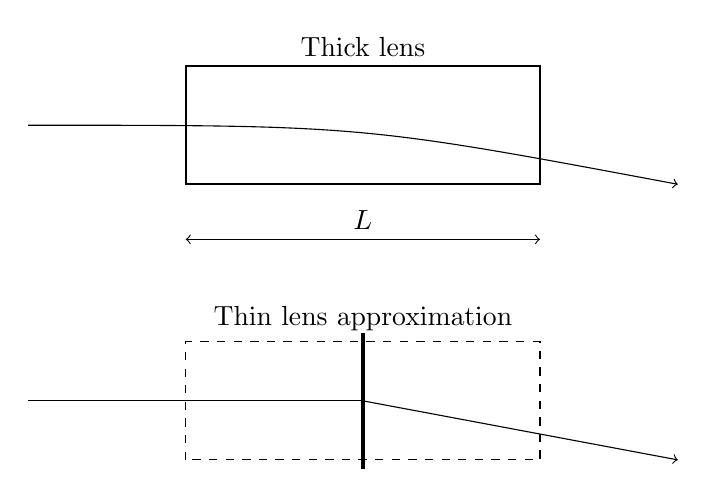
\begin{tikzpicture}
%    \draw[black,thin] (0.0,0.0) grid (16.0,9.0);

    % thick lens 
    \draw[thick] (6.0,4.5) rectangle (10.5,6.0);
    \draw[->] (4.0,5.25) .. controls (8.25,5.25) .. (12.25,4.5);
    \node [rotate=0]  at (8.25,6.25)    {Thick lens};


    %  thin lens
    \draw[dashed]      (6.0,1.0) rectangle (10.5,2.5);
    \draw[<->] (6.0,3.8) -- (10.5,3.8);
    \node [rotate=0]  at (8.25,4.05)    {$L$};

    \draw[thick] (8.24,0.9) rectangle (8.26,2.6);
    \draw (4.0,1.75)  -- (8.25,1.75);
    \draw[->] (8.25,1.75) -- (12.25,1.0);
   \node [rotate=0]  at (8.25,2.80)    {Thin lens approximation};


   
  \end{tikzpicture}
  \caption{Schematic illustration of the thin lens approximation. The transverse bending of a magnet of length $L$ is approximated by a point-like kick the particle receives only at the center of the magnet. Left and right of the magnet center the transverse particle momentum remains unchanged.}
  \label{pic:thinlens}
\end{figure}









The analytic treatment of the transfer matrices can be significantly simplified if the magnet length $L$ is small compared to $1/KL$. The magnetic bending can then be treated as a point-like transverse kick which is given to the particle at the center of the magnet. In the rest of the element length, the particle trajectory remains undisturbed, hence behaves like a drift space (see \figref{pic:thinlens}). Mathematically, this thin lens approximation~\cite{CERN-SL-95-12} corresponds to the limit
\begin{align}
  L \rightarrow 0 \quad \text{with} \quad K \, L = \text{const.} 
\end{align} 
The transfer matrix for a quadrupole magnet simplifies in the thin lens approximation to
\begin{align}
  \mathcal{M}_{Q,f/d} = \begin{pmatrix}  1 & L \\   KL & 1  \end{pmatrix} \, ,
\end{align}
which is equivalent to the transfer matrix of a thin optical lens with focal length $f=\frac{1}{KL}$.
%
\subsubsection{Periodic Solution and Betatron Motion}
An alternative to the solution of the homogeneous part of the equation of motion, given before in matrix form, is given by
%
\begin{align}
x(s) = \sqrt{\tilde{\epsilon}_x} \, \sqrt{\beta_x(s)} \, \cos \left( \psi_x(s) + \phi \right) \, , \label{eq:betatron_oscillation}
\end{align}
%
where $\tilde{\epsilon}$ and $\phi$ are mathematically the integration constants and represent the initial conditions of the particle. The function $\beta_x(s)$ is called the betatron function. The latter is related to the maximum amplitude the particle trajectory can take at the position $s$. 

\newpage
In circular accelerators the quantity $K(s)$ is periodic with the same period as the machine circumference $C$
\begin{align}
K(s) = K(s+C) .
\end{align}
The equation of motion (\ref{eq:hill1}) with periodic $K(s)$ is the Hill differential equation~\cite{wiedemann1999particle}. The solution of Hill's equation is identical to \eqref{eq:betatron_oscillation}, but the periodicity implies that also $\beta_x(s)$ is periodic in $s$ with period $C$
%
\begin{align}
  \beta_x (s) = \beta_x (s+C) \, .
\end{align}
The betatron function is purely defined by the magnetic lattice in the accelerator. The particles perform transverse quasi-harmonic oscillations in $x$, around the ideal trajectory. The local amplitude of these so-called betatron oscillations is defined by $\tilde{\epsilon}_x$, the betatron function $\beta_x(s)$ and the betatron phase $\psi_x(s)$, defined as
%
\begin{align}
  \psi_x(s) = \int_0^s \frac{\mathrm{d}s}{\beta_x(s)} \, .
\end{align}
%
The total number of betatron oscillations over one turn is called the machine tune
%
\begin{align}
  Q_x = \frac{1}{2 \pi} \int_0^C \frac{\mathrm{d}s}{\beta_x(s)} \, .
\end{align}
%
%
From \eqref{eq:betatron_oscillation} and its derivative, it can be deduced that $\tilde{\epsilon}_x$ is a constant of motion, mathematically the Courant-Snyder invariant, for the individual particle and can be expressed as
%
\begin{align}
\tilde{\epsilon}_x = \gamma_x(s) \, x^2(s) + 2 \, \alpha_x(s) \, x(s) \, x'(s) + \beta_x(s) \, x'^2 (s) \, . \label{eq:parameric_ellipse}
\end{align}
%
The quantities $\beta_x(s)$, $\alpha_x(s)$ and $\gamma_x(s)$ are the so-called Twiss parameters~\cite{wiedemann1999particle}. They are defined by the magnetic lattice in the machine which transforms the beam equivalently to a lattice of lenses in classical optics. The Twiss parameters are therefore also referred to as the optical functions, and the configuration of the magnetic lattice as the beam optics.

The derivative of the betatron function $\beta_x(s)$ defines the two remaining Twiss parameters as
\begin{align}
\alpha_x(s) = - \frac{1}{2} \beta_x'(s) \quad \quad \gamma_x(s) = \frac{1+\alpha_x(s)^2}{\beta_x(s)} \, .
\end{align}

%
\begin{figure}[b]  
    \centering
    \includegraphics[width=1\textwidth]{pictures/16021801.pdf}
    \caption{Individual particle trajectories in a periodic quadrupole lattice.}  
    \label{pic:16021801}
    %/home/phermes/Dropbox/PhD/pictures/160217_beam_enveloppe/enveloppe.pdf
\end{figure}

The evolution of an initial set $(\alpha_{x,0},\beta_{x,0},\gamma_{x,0})$ of Twiss parameters in the accelerator depends on the lattice elements and is, equivalent to the transformation of the particle coordinates in \eqref{eq:transfer_matrix}, described by their transfer matrices as follows
%
\begin{align}
  \beta_x(s) = C_x^2 \, \beta_{x,0} -2 \, S_x^2 \, C_x^2 \, \alpha_{x,0} + S_x^2 \, \gamma_{x,0} \, .
\end{align}
%
Furthermore, the expression in \eqref{eq:parameric_ellipse} is the parametric representation of an ellipse in $x,x'$ enclosing a phase space surface of $\pi \tilde{\epsilon}_x$. Shape and orientation of the phase space ellipse are changing as a function of the Twiss parameters. The surface in phase space that is enclosed by the ellipse remains unchanged if only conservative forces act on the beam particles (Liouville's theorem)~\cite{wiedemann1999particle}. Following \eqref{eq:betatron_oscillation}, the largest possible amplitude in $x$ and $x'$ the individual particle can reach yields (see \figref{pic:ell}):
%
\begin{align}
  x_\text{max} = \sqrt{\tilde{\epsilon}_x \, \beta_x(s)} \quad \text{and} \quad x_\text{max}' = \sqrt{\tilde{\epsilon}_x \, \gamma_x} \, .
\end{align}
%
The quantity $x_\text{max}$ is hence related to the peak amplitude of the betatron oscillation for a given $\beta$-function. If many particles compose the beam, the RMS value of the individual $\tilde{\epsilon}_x$ is referred to as the emittance, which is directly related to the RMS beam size $\sigma_x(s)$:
%
%
\begin{figure}[t]  
  \centering
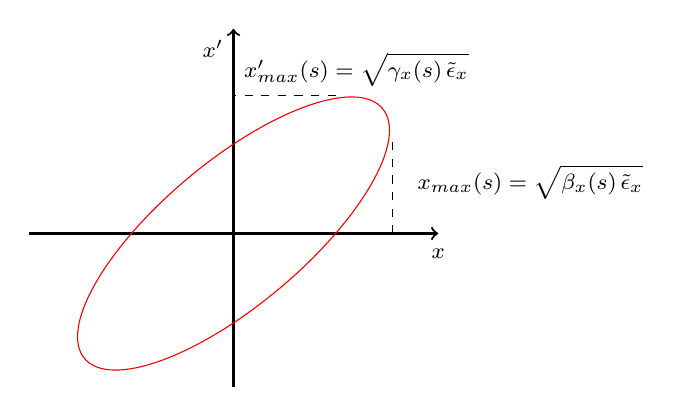
\begin{tikzpicture}[scale=1.3]
  \footnotesize
  % helper grid: comment for final drawing
  % \draw[help lines,step=.2] (0,0) grid (16.0,9.0);
  % \draw[help lines,line width=.6pt,step=1] (0,0) grid (16.0,9.0);
  % \foreach \x in {0,1,2,3,4,5,6,7,8,9,10,11,12,13,14,15,16}
  %      \node[anchor=north] at (\x,-0.1) {\x};
  % \foreach \y in {0,1,2,3,4,5,6,7,8,9}
  %     \node[anchor=east] at (-0.2,\y) {\y};

  % % text
  % \node [draw,rotate=90]  at (3.50,5.50)  {Injection};
  % % straight line and parabola
  % \draw [red,thick]          (0,0) -- (4,3);
  % \draw [black,thick,dashed] (0,0) parabola (4,4);
  % % bezier lines
  % \draw (6,0) .. controls (6,4) and (10,0) .. (10,4);
  % % circular shapes
  % \draw (5,5) circle (2cm);
  % \draw (7,2) ellipse (3cm and 1cm);
  % \draw (3,5) arc (0:75:3cm);
  % % filled rectangle



  % lower blms
%  \filldraw[fill=orange, draw=black] (9.2,3.8) rectangle (9.6,4.0);



  % % axes
  \draw[->,thick] (5,1.5) -- (5,5);
  \draw[->,thick] (3,3) -- (7,3);

  \draw[rotate around={40:(5,3)},red] (5,3) ellipse (1.9 and 0.7);

  % \draw[->,thick] (3.5,1) -- (3.5,4);
  % \draw[dashed] (3.5,2.0) circle (1.0);
  % \draw[red,thick,->] (3.5,3.0) arc (90:40:1.0);
  % \draw[red,thick,-] (3.5,3.0) arc (90:130:1.0);

  % \draw[->,thick] (3.5,2) -- (3.9,2.9);
  \draw[dashed] (6.55,3) -- (6.55,3.9);
  \draw[dashed] (6.0,4.35) -- (5.0,4.35);
  \node  at (7.9,3.5)  {$x_\text{max}(s) = \sqrt{ \beta_x(s) \, \tilde{\epsilon}_x}$};
  \node  at (6.2,4.6)  {$x_\text{max}'(s) = \sqrt{ \gamma_x(s) \, \tilde{\epsilon}_x}$};
  % \node  at (3.9,2.4)  {$\rho_0$};
  % \node  at (4.4,2.8)  {$S$};
  % \node  at (5.0,2.8)  {$z$};
  \node  at (7.0,2.8)  {$x$};
  \node  at (4.8,4.8)  {$x'$};
  % \node  at (4.3,3.4)  {$X$};

  % \draw[thick,->] (0,0) -- (0,4.5);

\end{tikzpicture}
  \caption{Phase space ellipse with $x_\text{max}$ and $x_\text{max}'$.}
  \label{pic:ell}
  \end{figure}
%
%
%
\begin{align}
  \sigma_x (s) = \sqrt{\epsilon_x \, \beta_x} \quad \text{with} \quad \epsilon_x = \langle \tilde{\epsilon_x} \rangle_{\text{rms}} \, .
\end{align}
%
The quantity $\sigma_x(s)$ defines an RMS beam envelope at the position $s$ which contains $1 \, \sigma_\text{rms}$ of the beam particles. In \figref{pic:16021801}, the betatron motion of particles with different initial conditions within $\epsilon_x$ is shown in a periodic lattice of quadrupoles and bending dipoles. It is clearly visible how the individual particle tracks are confined by $\sigma_x$.
%

The emittance is a measure for the beam quality and should be as small as possible. If the particle beam is accelerated, only the longitudinal momentum is increased. It can be shown that the ratio of transverse momentum to longitudinal momentum decreases $\frac{1}{\beta \, \gamma}$, which is referred to as adiabatic damping~\cite{wiedemann1999particle}. Consequently, the normalized horizontal emittance is defined as 
%
\begin{align}
  \epsilon_N = \epsilon_x \, \beta \gamma \, ,
\end{align}
and remains constant for all particle energies, assuming that, besides the acceleration, only conservative forces  act on the beam. The emittance is measured in units of $\mu$m rad.




\subsubsection{Solution of the inhomogeneous Equation of Motion}


The solution of the inhomogeneous equation of motion \eqref{eq:hill1} can be expressed as
%
\begin{align}
  x(s) = x_h(s) + x_i(s) \, , \label{eq:inhsol}
\end{align}
%
where $x_h(s)$ is the solution of the homogeneous equation shown in \eqref{eq:general_solution} and $x_i$ is one particular solution of the inhomogeneous equation, for example
%
\begin{align}
  x_i(s) = \bar{D}_x(s) \, \delta \, .
\end{align}
%
The dispersion function $\bar{D}_x(s)$ is a periodic function in $s$ with period length $C$, depending on the magnetic elements in the entire ring. It is defined as
%
\begin{align}
  \bar{D}_x (s) = - \frac{\beta_x(s)}{2 \, \sin (\pi \, Q_x)} \, \int_{s_0}^{s_0+C} \, h_x(\tilde{s}) \, \sqrt{\beta(\tilde{s})} \, \cos \left[ 2 \pi \, \left( \psi(\tilde{s}) - \psi(s_0) - \frac{Q_x}{s} \right) \right] \, \mathrm{d} \tilde{s} \, .
\end{align}

In order to be coherent with the definition in the simulation tools used, in the following the dispersion function will be expressed in terms of $D_x(s)$, defined as
%
\begin{align}
  D_x(s) = -\bar{D}_x(s) \, . \label{eq:dispoff}
\end{align}
%
As shown in \eqref{eq:inhsol}, the dispersion function relates the momentum offset of the particle to an additional transverse amplitude. The quantity $D_x (s) \, \delta$ hence gives the closed orbit around which  off-momentum particles perform betatron oscillations. For multi-isotopic beams, \eqref{eq:dispoff} still applies, but the relative momentum offset is replaced by $\delta_\text{eff}$.

It is often useful to also define the local dispersion function $\tilde{D}_x(s)$, which quantifies the dispersive offset an off-rigid particle acquires between two defined locations. This becomes important, when the rigidity of a particle changes at a given location and the particle trajectory should be followed from the location at which the rigidity offset was acquired.

Note that this mathematical description represents a linear approximation and higher order dispersive effects are not taken into account. For particles with large momentum offsets, a more accurate description is given by a fully symplectic transformation without truncation, which can be derived from the accelerator Hamiltonian (see \chapref{chap:hamiltonian}). 



\section{Longitudinal Particle Dynamics}

\input{pictures/cavity.tex}

The beams in the LHC are accelerated and longitudinally confined by means of radio frequency cavities (RF cavities)~\cite{wiedemann1999particle}. They consist of a periodic resonator structure (illustrated in \figref{pic:cavity}) and are operated with RF waves and provide a longitudinal electric field $V(t)$ of a defined frequency $\phi_\text{RF} = \omega_\text{RF} \, t$
%
\begin{align}
  V(t) = V_0 \, \sin (\phi_\text{RF} + \phi_s) \, ,
\end{align}
%
where $V_0$ is the peak amplitude of the electric field and $\phi_s = \omega_s \, t$ is the phase of the synchronous particle. The frequency of the RF cavity is adapted to the revolution frequency $f_\text{rev}$ of the synchronous particle, to provide the same accelerating voltage at every turn
%
\begin{align}
  f_\text{RF} = h \, f_\text{rev} \, ,
\end{align}
%
where $h$ is the harmonic number. Assuming that $q=q_0$, the energy $\Delta E$ transferred to a particle arriving at phase $\phi$ compared to the phase of the synchronous particle $\phi_s$ is given by~\cite{CAS2013}
%
\begin{align}
  \Delta E =  q_0 \, V_0 \, \left( \sin \phi - \sin \phi_s \right) \, .
\end{align}
%
The phase dependence of the energy transfer leads to a different energetic kick for particles arriving at different times than the synchronous particle. If $\phi_s$ is correctly chosen, particles with momentum $P$ smaller than the reference momentum $P_0$ (which arrive with time delay), receive a larger momentum transfer and those with $P>P_0$ receive a smaller momentum transfer than the synchronous particle. This is illustrated in the top plot of \figref{pic:16081703}. 

It can be shown~\cite{CAS2013} that the difference in phase $\Delta \phi = \phi - \phi_s$ with respect to the reference particle obeys the differential equation
%
\begin{align}
  \frac{ \mathrm{d}^2}{\mathrm{d} t^2 } \phi + \frac{\Omega_s^2}{\cos \phi_s} \, ( \sin \phi - \sin \phi_s ) = 0 \quad \text{with} \quad \Omega_s^2 = \frac{h \, \eta \, \omega_\text{rs} \, q_0 \, V_0 \, \cos \phi_s}{ C \, P_0} \, . \label{eq:syncmo}
\end{align}
Here, $h$ is the harmonic number, $\eta = \frac{\Delta \omega_\text{r}/\omega_\text{rs}}{\Delta P / P_0}$ is the slip factor which quantifies the change in revolution frequency implied by a change in momentum, $\omega_\text{rs}$ is the revolution frequency of the synchronous particle and $C$ is the circumference of the machine. 


\begin{figure}[t]
  \centering
  \begin{tikzpicture}
    \node[anchor=south west,inner sep=0] (image) at (0,0) {\includegraphics[width=0.6\linewidth]{pictures/16081703.png}};
    %\node [draw,rotate=90,x={(image.south east)},y={(image.north west)}]                   at (0.50,0.50)    {text0};
    %\node [draw,rotate=0 ,x={(image.south east)},y={(image.north west)}]                   at (0.22,0.96)    {text1};
    %\node [draw,rotate=0 ,x={(image.south east)},y={(image.north west)},anchor=west]       at (0.22,0.80)    {text2};
    %\draw[->,color=black,thick,x={(image.south east)},y={(image.north west)}]             (0.42,0.22) -- (0.37,0.23);
  \end{tikzpicture}
  \caption{Top panel: longitudinal electric field $V$ as a function of the particle phase $\phi$. Particles with $P<P_0$ which arrive later than the reference particle (1) receive a larger energy transfer. Accordingly, particles arriving before the reference particle (2) receive a smaller energetic kick. The particles perform an oscillation in the $\phi, \frac{\Delta P}{P_0}$-plane (bottom panel). The stable region in $\phi, \Delta P/P_0$ is defined by a separatrix. Figure courtesy of \cite{CAS2013}.}  
  \label{pic:16081703}
  %/home/phermes/Dropbox/PhD/thesis//home/phermes/Desktop/separartrix.png
  \end{figure}

For small phase deviations $\Delta \phi_s$, the expression in \eqref{eq:syncmo} can be simplified to~\cite{CAS2013}
%
\begin{align}
  \frac{ \mathrm{d}^2}{\mathrm{d} t^2 } \phi + \Omega_s^2 \,  \Delta \phi = 0 \, ,
\end{align}
which describes a harmonic oscillation (the so-called synchrotron oscillation) in $P$ and $\phi$, with frequency $\Omega_s$. Stability of the longitudinal motion implies that $\Omega_s^2>0$, which is the case when $\eta \, \cos \phi>0$, as illustrated in \figref{pic:16081703}.


Stable and unstable regions in the $\phi, \Delta P/P_0$ plane are separated by the so-called separatrix, which defines the largest amplitude in $\phi, \frac{\Delta P}{P_0}$ that is compatible with stable synchrotron oscillations. The region inside the separatrix is called RF bucket. 

By virtue of the periodicity of the electric field in the RF cavity, multiple buckets are available to store particles in the machine. The concrete number of buckets is determined by the harmonic number. Thus, the accelerating RF cavities imply a bunching of the particle beam. 




